\documentclass[UTF8]{ctexart}

\usepackage{subfiles}  

%下面的语句, 引入你的头部设置文件
\usepackage{C:/phpStorm_proj/02_myself_ID_EGO/+100_latex_all_math_sel/myPreamble} 
%必须是绝对路径,才能让各个tex在单独编译时使用到

\title{文件名}


%---------------------------------


\begin{document}
	\tableofcontents % 生成目录
	\date{} % 若不写这句, 则默认也会渲染出日期, 所以我们要手动赋空值
	\maketitle  %这行代码, 让你前面的 title, author, date生效
	
	
	
	
	\part{交集 $\cap$ , 与 并集 $\cup$}
	
	
	\section{表``或", 用加法(+); 表``同时", 用乘法(×)}
	
	A, B, C 是 试验E 的随机事件. 则表示法是:
	
	- A发生 : $A$ \\
	
	下面, 加法即表示``或" :
	
	- A, B, C 恰有一个发生 : $A\overline{B}\overline{C}+\overline{A}B\overline{C}+\overline{A}\overline{B}C$
	
	- A, B, C 至少一个发生(即 >=1) : A+B+C 或 $A{\cup}B{\cup}C$ ← 即3选1, 还有两个发不发生, 不用管, 随意, 都行.
	
	- A, B, C 至多一个发生(即 <=1) : $\underset{3\text{选}1}{\underbrace{A\overline{B}\overline{C}+\overline{A}B\overline{C}+\overline{A}\overline{B}C}}+\underset{3\text{选}0}{\underbrace{\overline{A}\overline{B}\overline{C}}}		$
	
	- 恰有两个发生: $AB \overline{C} + A \overline{B} C + \overline{A} BC $
	
	- 至少两个发生(即,>=2 ) : $\underset{3\text{选}2}{\underbrace{AB\overline{C}+A\overline{B}C+\overline{A}BC}}+\underset{3\text{选}3}{\underbrace{ABC}}+\underset{3\text{选2,\ 还有一个发不发生不用管,随意}}{\underbrace{AB+BC+AC}}	$	\\
	
	
	
	下面, 乘法即表示``同时" :	
	
	- 只有A发生 : $A\overline{B}\overline{C}$	
	
	- A, B, C 同时发生 : ABC  \\
	
	\begin{myEnvSample}
		一次射击试验, 整个流程是打三枪, 用 $A_i, (i=1,2,3)$ 来表示``在第i次时击中了目标".
		
		记住: 加法(+) 代表``或,并 $\cup$"; 乘法代表``交$\cap$".
		
		- $A_1+A_2$ : 表示第一次击中了, 或第二次击中了. 即前两次至少击中一次.
		
		- $	\overline{A_2}	$ : 表示第二次没击中.
		
		- $	A_1+A_2+A_3	$ : 表示仅第一次击中, 或仅第二次击中, 或仅第三次击中.
		
		- $	A_1A_2A_3	$ : 表示三次全中.
		
		- $	A_2\overline{A_3} = A_2 - A_3	$ : 表示第二次击中, 并且第三次失败.
		
		- $	\overline{A_1}\cap \overline{A_3}=\overline{A_1+A_3}$ : 表示第一次没中, 并且第三次也没中.
		
		- $	\overline{A_1}+\overline{A_3}	$ : 表示第一次没中, 或第三次没中.
		
		
	\end{myEnvSample}
	
	
	
	
	\section{公理化}
	
	\subsection{$P(A) + P(\overline{A}) = 1$}
	
	\subsection{对于``完备事件组"中的所有事件来说: $P(A_1) + P(A_2) + ... +  P(A_n) =  P(\Omega) = 1$}
	
	完备事件组 collectively exhaustive events 就是: 如果事件 B1, B2, B3, ...  Bn 满足:
	
	1. 它们两两互不相容(即两两的交集=空集),
	
	2. 其``和"为全集 Ω. 	
	
	换言之, 若n个事件两两互斥, 且这n个事件的``并"是 Ω,则称这n个事件为``完备事件组". \\
	
	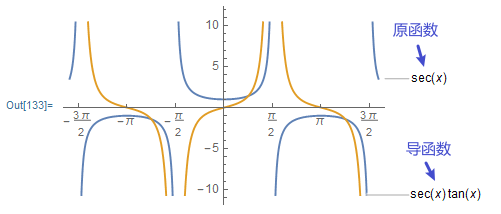
\includegraphics[width=0.6\textwidth]{/0069.png}
	
	
	\begin{myEnvSample}
		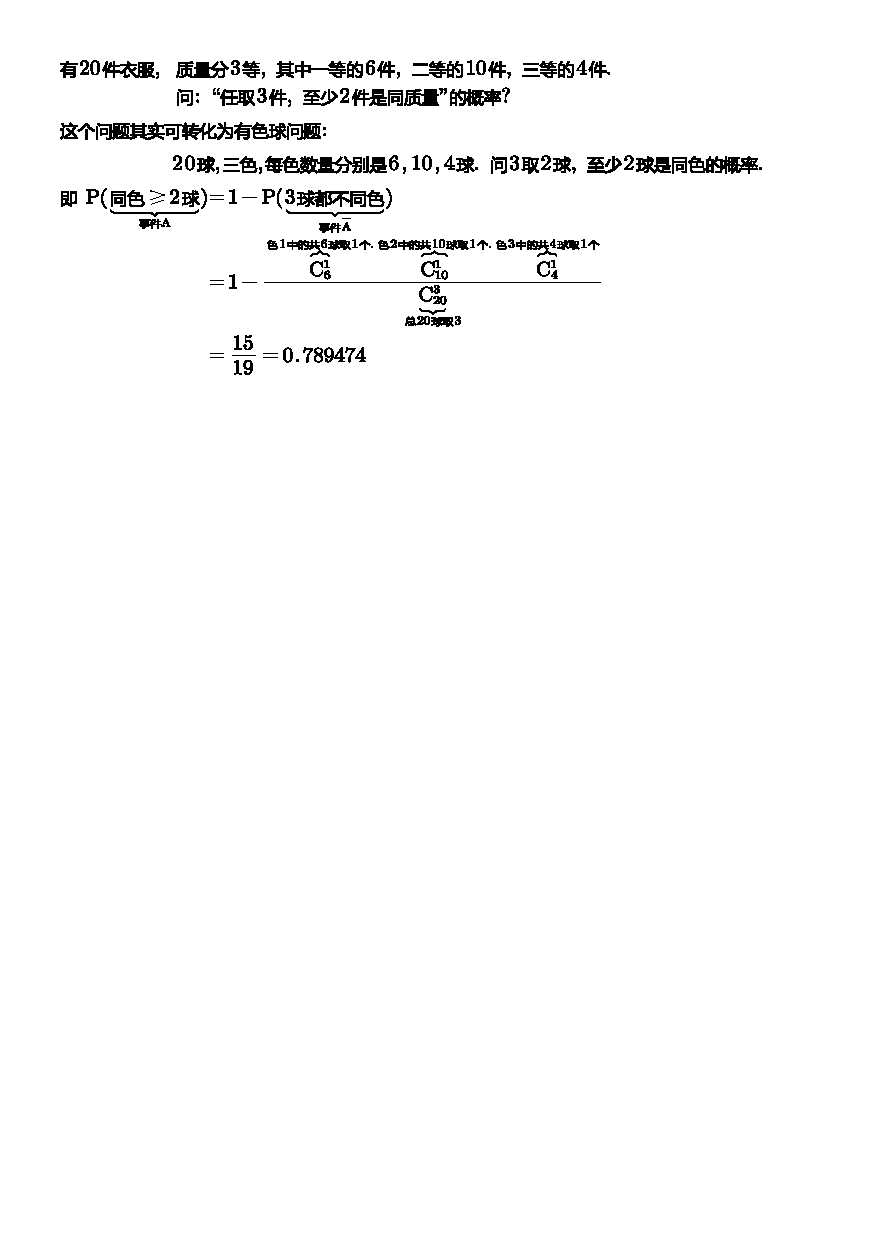
\includegraphics[width=0.9\textwidth]{/0076.pdf} \\
		
		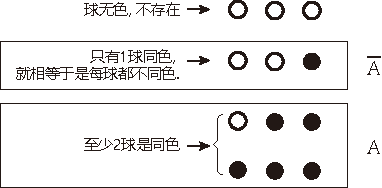
\includegraphics[width=0.5\textwidth]{/0077.pdf}
	\end{myEnvSample}
	\vspace{1em} 
	
	
	\begin{myEnvSample}
		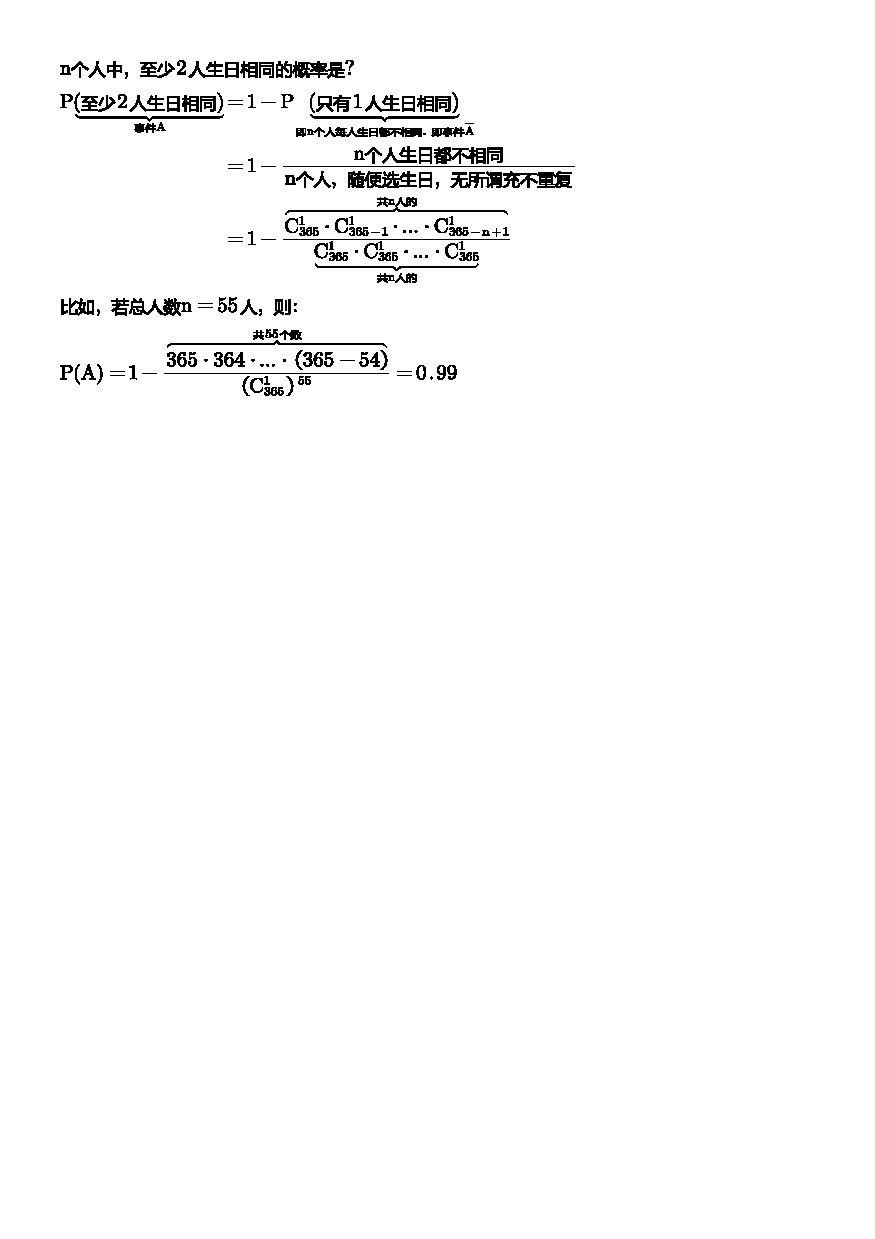
\includegraphics[width=0.65\textwidth]{/0079.pdf} \\
		
		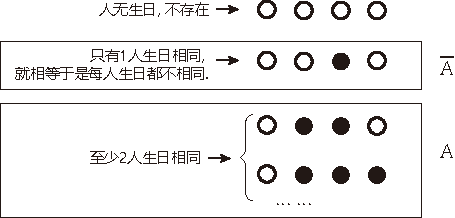
\includegraphics[width=0.6\textwidth]{/0078.pdf} 
	\end{myEnvSample}
	
	
	
	\subsection{$P(A-B) = P(A) - P(AB)$}	
	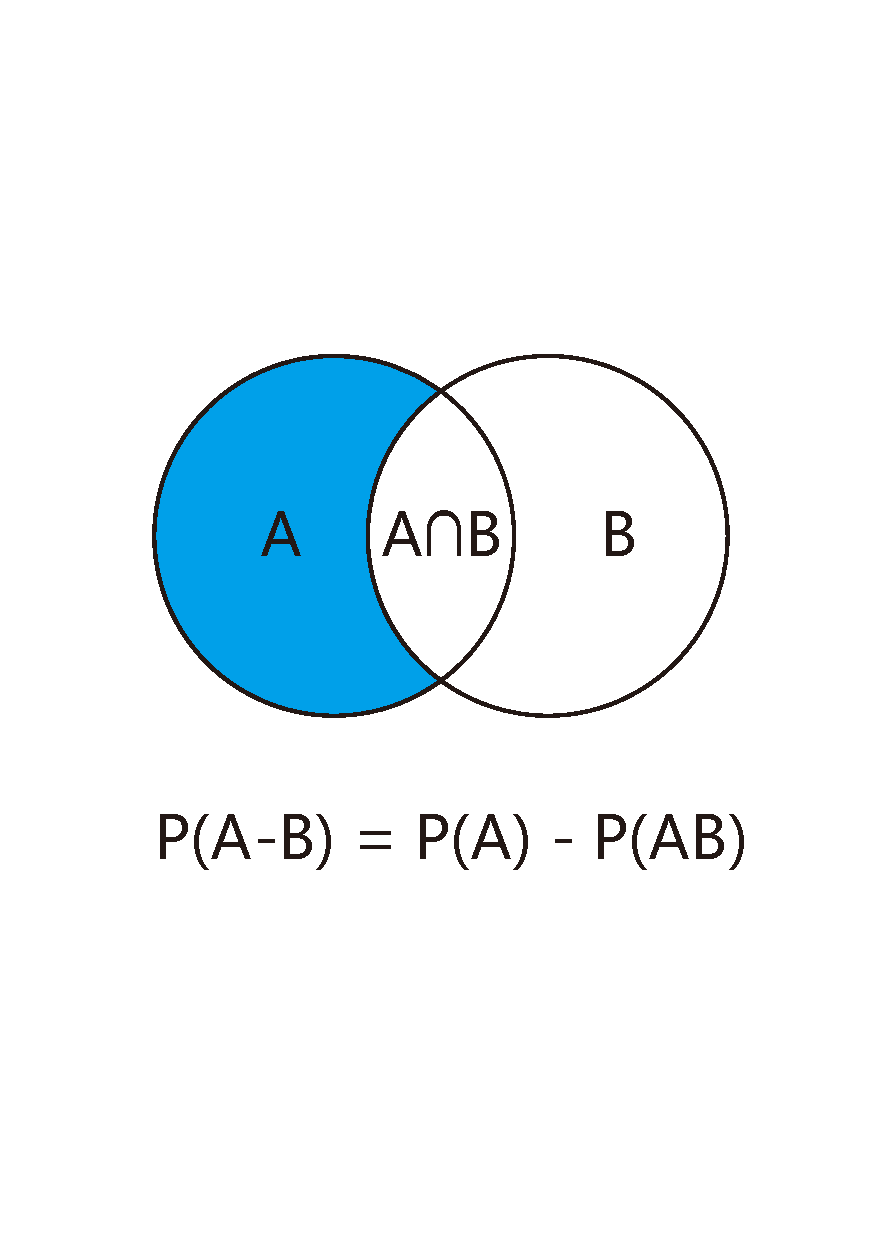
\includegraphics[width=0.2\textwidth]{/0070.pdf}
	
	
	\subsection{若A包含着B, 则有: $ P(A-B) = P(A) - P(B)$, 且 $P(A) >= P(B) $}
	
	
	\subsection{加法公式: $ P(A+B) = P(A) + P(B) - P(AB)$}	
	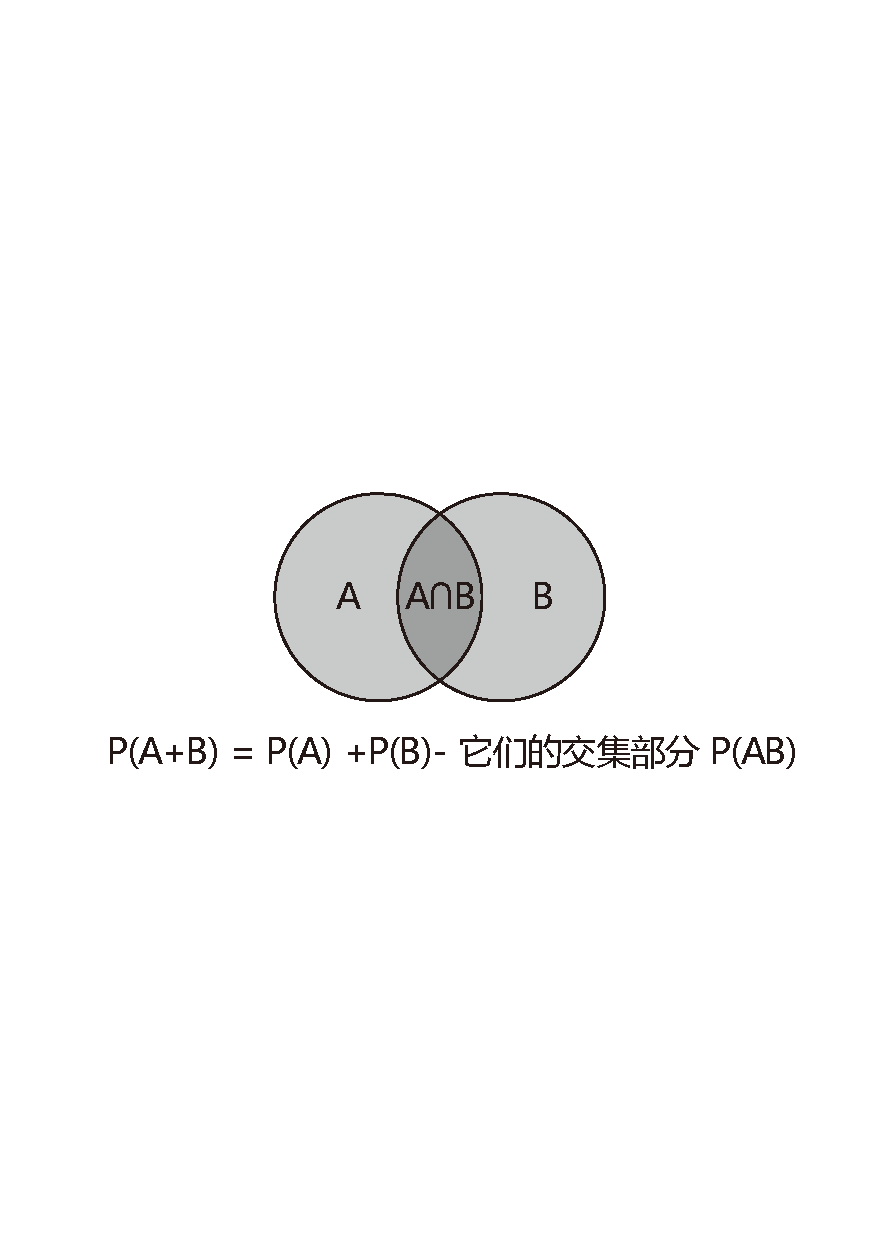
\includegraphics[width=0.4\textwidth]{/0071.pdf} \\
	
	\begin{myEnvSample}
		A事件的概率是0.4, 即 P(A)=0.4; 
		
		P(B)=0.3; 
		
		且P(A+B)=0.6, ← 说明A与B有交集部分存在. 否则, 如果A与B是不相容的话, 它们和的概率, 应该是 0.4+0.3=0.7.
		
		所以它们的交集 P(AB) 就是=0.1 : 
		
		$
		\underset{0.6}{\underbrace{P\left( A+B \right) }}=\underset{0.4}{\underbrace{P\left( A \right) }}-\underset{0.3}{\underbrace{P\left( B \right) }}-\underset{=0.1}{\underbrace{P\left( AB \right) }}
		$ \\
		
		求$P\left( A\overline{B} \right)$, 即求$A \cap B\text{逆}$ 的概率: 
		
		$
		P\left( A\cap \overline{B} \right) =P\left( A-B \right) =\underset{=0.4}{\underbrace{P\left( A \right) }}-\underset{=0.1}{\underbrace{P\left( AB \right) }}=0.3
		$ \\
		
		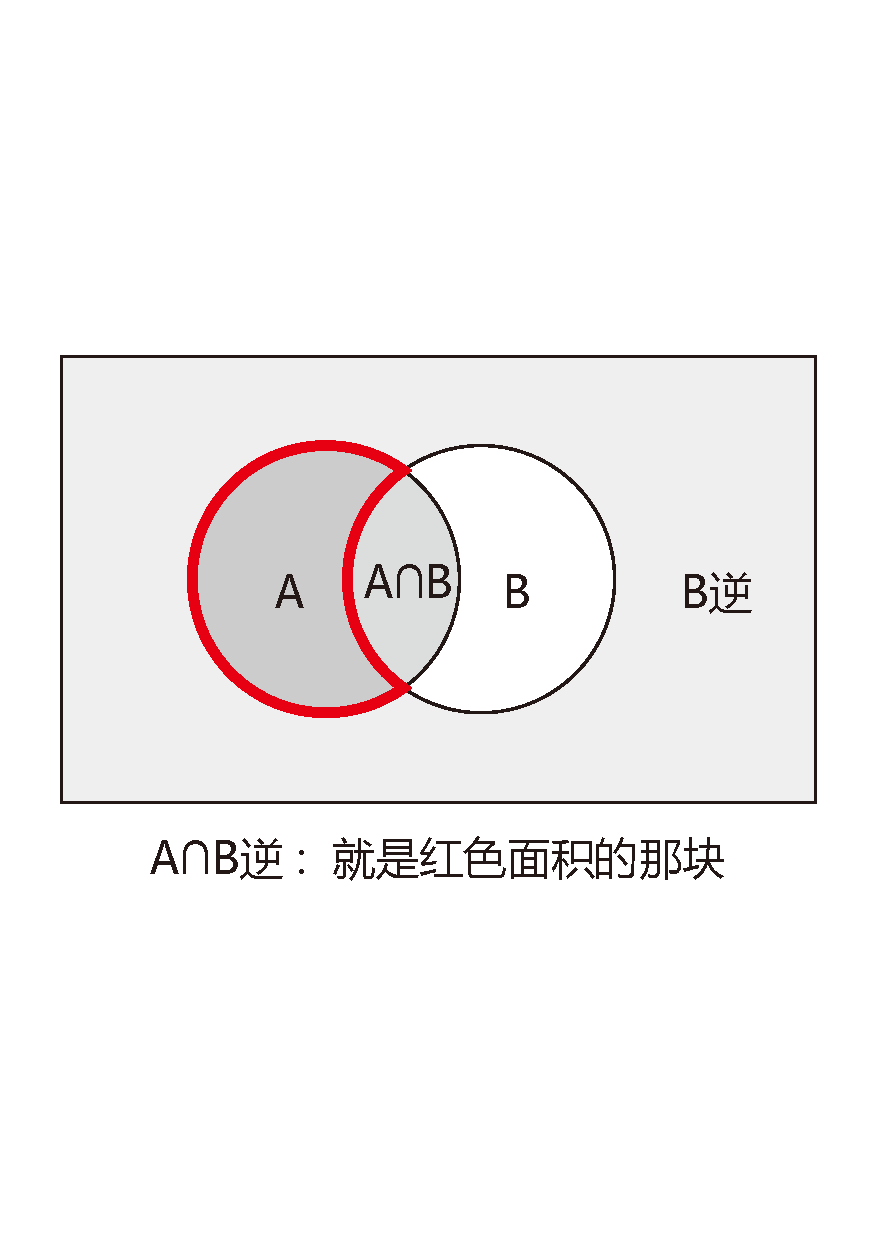
\includegraphics[width=0.35\textwidth]{/0073.pdf}
		
	\end{myEnvSample}
	
	
	
	
	
	\subsection{加法公式: $ P(A+B+C) = P(A) + P(B)  +  P(C) - P(AB) - P(AC) -  P(BC) +  P(ABC)$}
	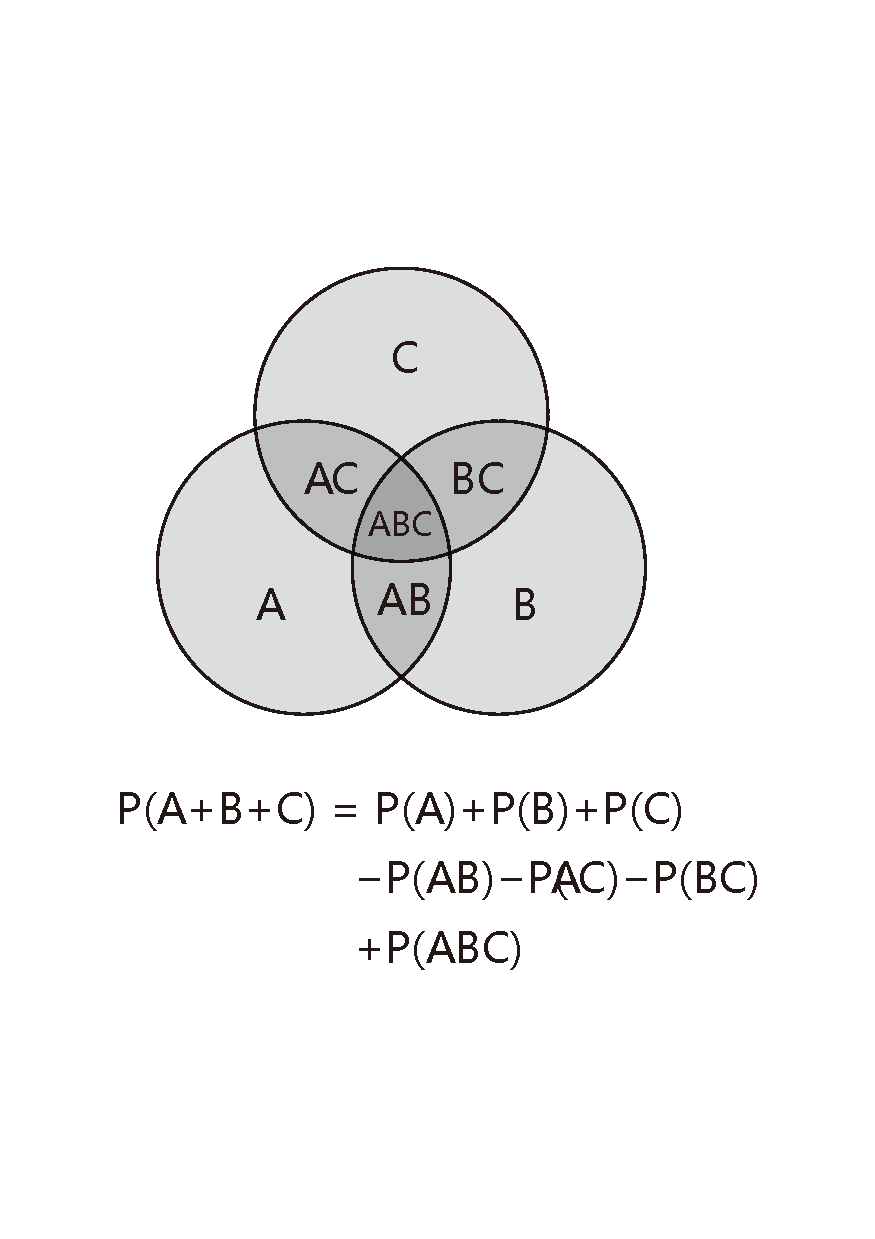
\includegraphics[width=0.3\textwidth]{/0072.pdf}	
	
	说明: 
	\begin{align*}  % 支持每行编号. 若不需要编号, 就用 align*环境
		& P\left( A+B+C \right) \\
		&=\underset{\text{这里,}ABC\text{交集部分,被加了3次}}{\underbrace{P\left( A \right) +P\left( B \right) +P\left( C \right) }}\underset{\text{这里,}ABC\text{交集部分,又减了3次}}{\underbrace{-P\left( AB \right) -P\left( AC \right) -P\left( BC \right) }}+\underset{\text{所以最后,我们还要把镂空的}ABC\text{交集部分,加上一份上去}}{\underbrace{P\left( ABC \right) }}
	\end{align*}
	
	
	\begin{myEnvSample}
		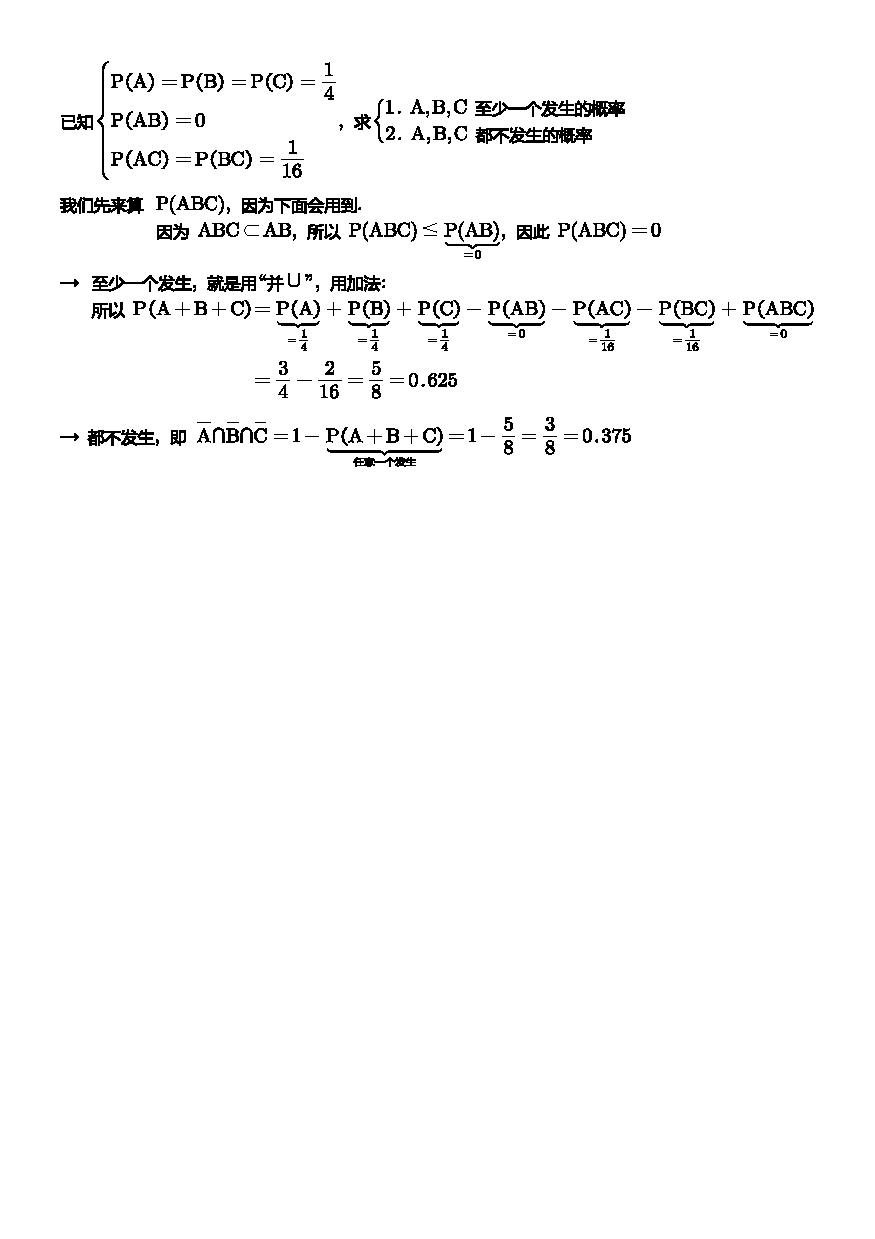
\includegraphics[width=1\textwidth]{/0074.pdf}
	\end{myEnvSample} 
	\vspace{1em} 
	
	
	\begin{myEnvSample}
		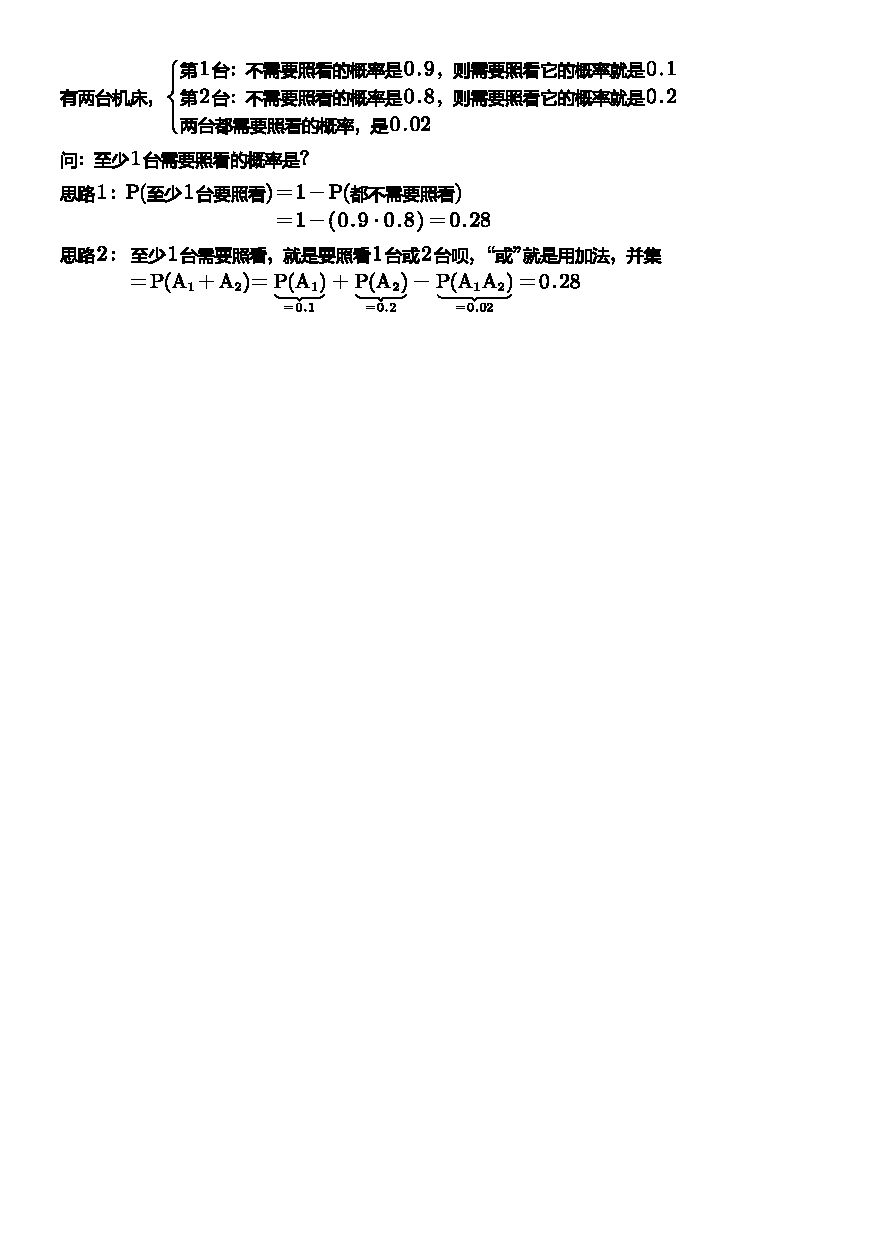
\includegraphics[width=0.82\textwidth]{/0075.pdf}
	\end{myEnvSample}
	
	
	
	
\end{document}